% !TeX program = xelatex
\documentclass[11pt,english]{article}
\usepackage[T1]{fontenc}
\usepackage{geometry}
\geometry{verbose,tmargin=2.5cm,bmargin=2.5cm,lmargin=2.5cm,rmargin=2.5cm}
\usepackage{color}
\usepackage{amsmath}
\usepackage{setspace}
\PassOptionsToPackage{normalem}{ulem}
\usepackage{ulem}
\usepackage{url}
\onehalfspacing
\usepackage{babel}
\usepackage{placeins}
\usepackage{float}

%\usepackage{mathtools}
\usepackage{fourier}            % set math font
%\usepackage{newpxmath}
\usepackage{bm} %bold math
\usepackage{fontspec}
\setmainfont{Times}
\setsansfont{Optima}
\renewcommand{\familydefault}{\sfdefault}
\usepackage{sectsty}
\allsectionsfont{\fontspec{Optima}}

%%%%%%%%%%%%%%%%%%%%%%%%%%%%%%%%%%%%%%%%%%%%%%%%%%%%%%%%%%%%%%%%%%%%%%%%%%%%%%%%%%%%%%%%%%%%%%%%%%%%%%%%%%%%%%%%%%%%%%%%%%%%
\usepackage{graphicx}
\usepackage{amsmath}

\setcounter{MaxMatrixCols}{10}
%TCIDATA{OutputFilter=LATEX.DLL}
%TCIDATA{Version=4.10.0.2345}
%TCIDATA{Created=Sat Aug 09 14:03:09 2003}
%TCIDATA{LastRevised=Wednesday, September 21, 2005 15:30:05}
%TCIDATA{<META NAME="GraphicsSave" CONTENT="32">}
%TCIDATA{<META NAME="DocumentShell" CONTENT="General\Blank Document">}
%TCIDATA{CSTFile=LaTeX article (bright).cst}

\newtheorem{theorem}{Theorem}
\newtheorem{acknowledgement}[theorem]{Acknowledgement}
\newtheorem{algorithm}[theorem]{Algorithm}
\newtheorem{axiom}[theorem]{Axiom}
\newtheorem{case}[theorem]{Case}
\newtheorem{claim}[theorem]{Claim}
\newtheorem{conclusion}[theorem]{Conclusion}
\newtheorem{condition}[theorem]{Condition}
\newtheorem{conjecture}[theorem]{Conjecture}
\newtheorem{corollary}[theorem]{Corollary}
\newtheorem{criterion}[theorem]{Criterion}
\newtheorem{definition}[theorem]{Definition}
\newtheorem{example}[theorem]{Example}
\newtheorem{exercise}[theorem]{Exercise}
\newtheorem{lemma}[theorem]{Lemma}
\newtheorem{notation}[theorem]{Notation}
\newtheorem{problem}[theorem]{Problem}
\newtheorem{proposition}[theorem]{Proposition}
\newtheorem{remark}[theorem]{Remark}
\newtheorem{solution}[theorem]{Solution}
\newtheorem{summary}[theorem]{Summary}
\newenvironment{proof}[1][Proof]{\textbf{#1.} }{\ \rule{0.5em}{0.5em}}
\oddsidemargin  0.2in
\textwidth      5.8in
\headheight     0.0in
\topmargin      -0.3in
\textheight=8.8in

\begin{document}

\title{Recitation 1 - Math Tools \thanks{Thanks to
    Professor Autor for sharing his lecture notes.}}
\author{Andrea Manera}
\date{14.03 Spring 2020}
\maketitle

\underline{\textbf{Agenda}}

\begin{itemize}
\item Optimization

\begin{itemize}
\item single variable

\item multi-variable
\end{itemize}

\item Implicit Function Theorem and comparative statics

\item Envelope Theorem: constrained and unconstrained

\item Constrained optimization (Lagrangian method)

\item Duality
\end{itemize}

\newpage

\bigskip

\section{Single Variable Optimization}

Suppose we can produce a unit of a good using a single unit of labor at a cost of $l^2$. That good sells for price $p$.  $\pi (q)=pq-q^2$ is the profit function and we choose $q^{\ast }$ to maximize $%
\pi (q)$

\bigskip

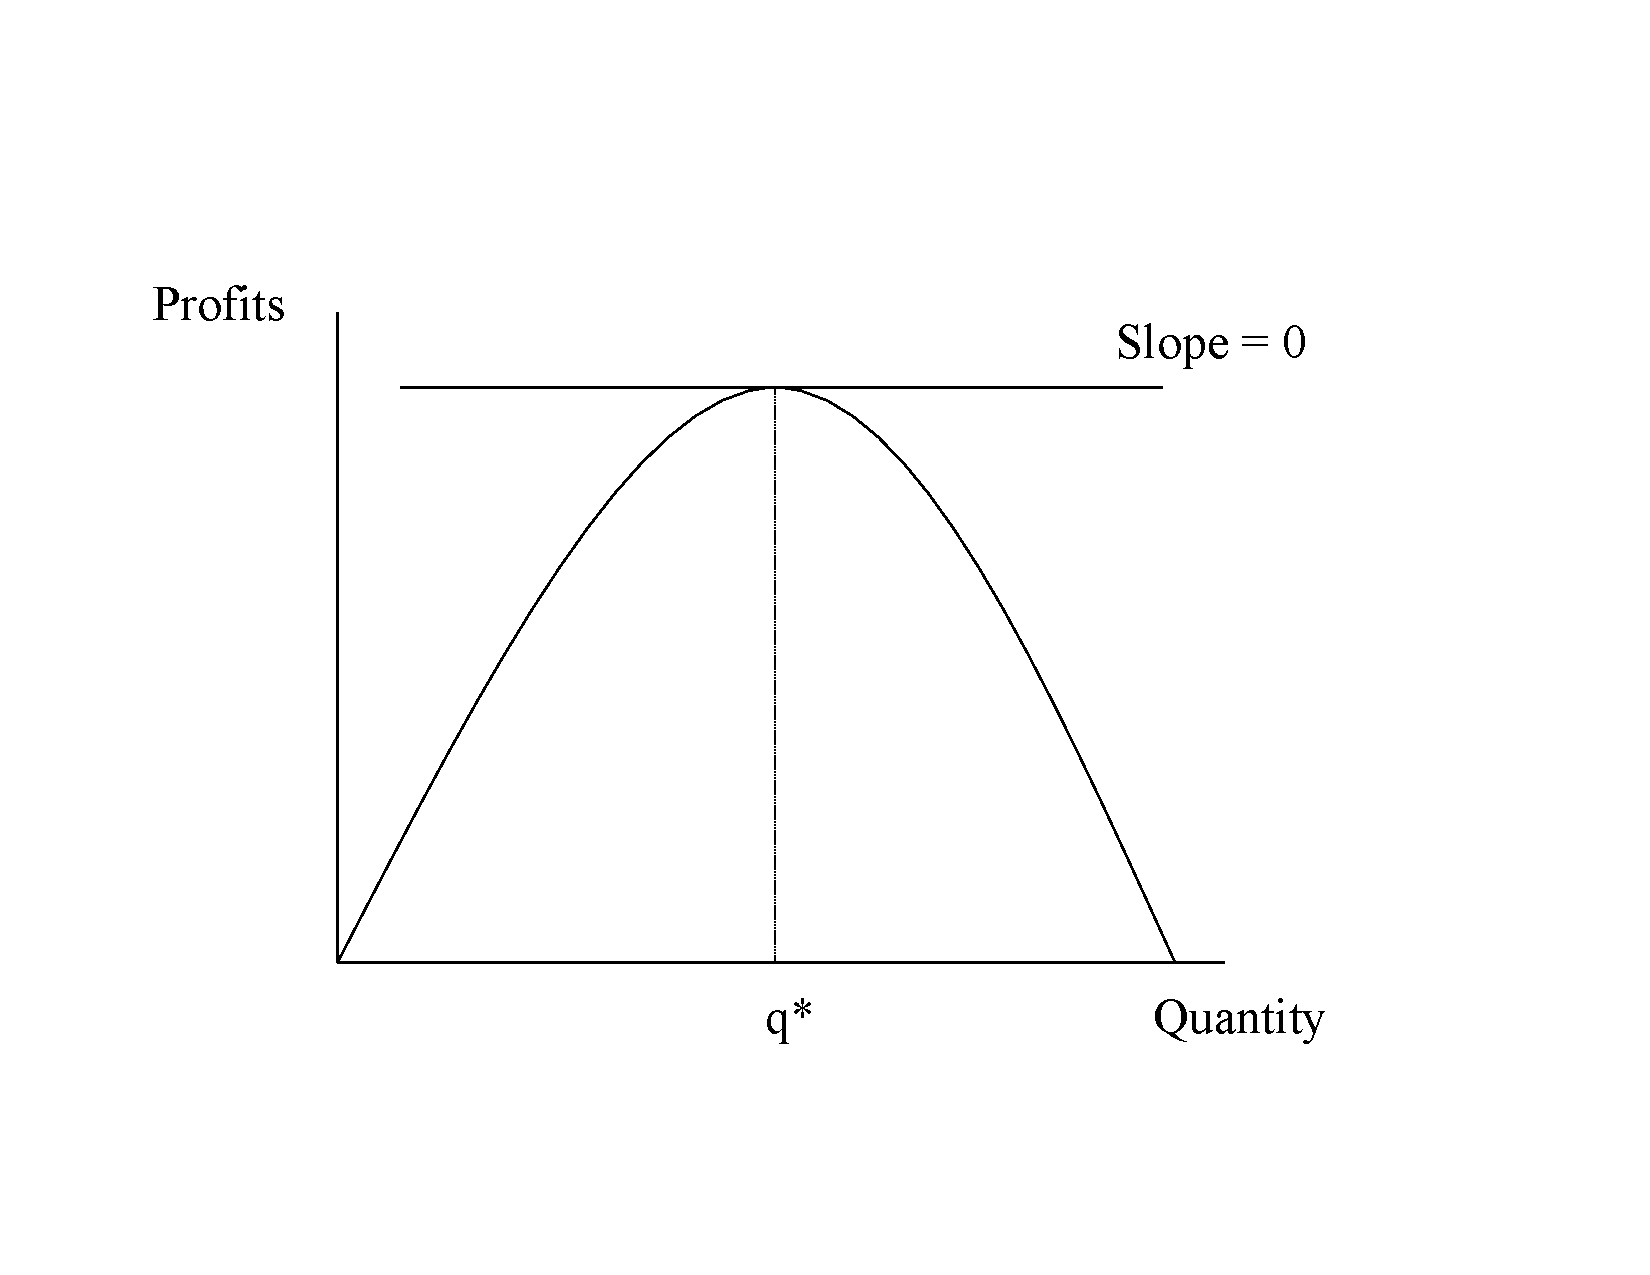
\includegraphics[scale=0.6]{math1.pdf}


\bigskip

First Order Condition (FOC):

\begin{eqnarray*}
\left. \frac{\partial \pi }{\partial q}\right| _{q^{\ast }}&=&0 \\
p-2q& = &0 \\ 
q^*(p)& = &\frac{p}{2}
\end{eqnarray*}

Q: Is $q^{\ast }$ necessarily the profit max?

A: No, FOC\ is necessary, but not sufficient for profit maximization. The
point that satisfies FOC could well be a minimum or an inflection point.

\bigskip
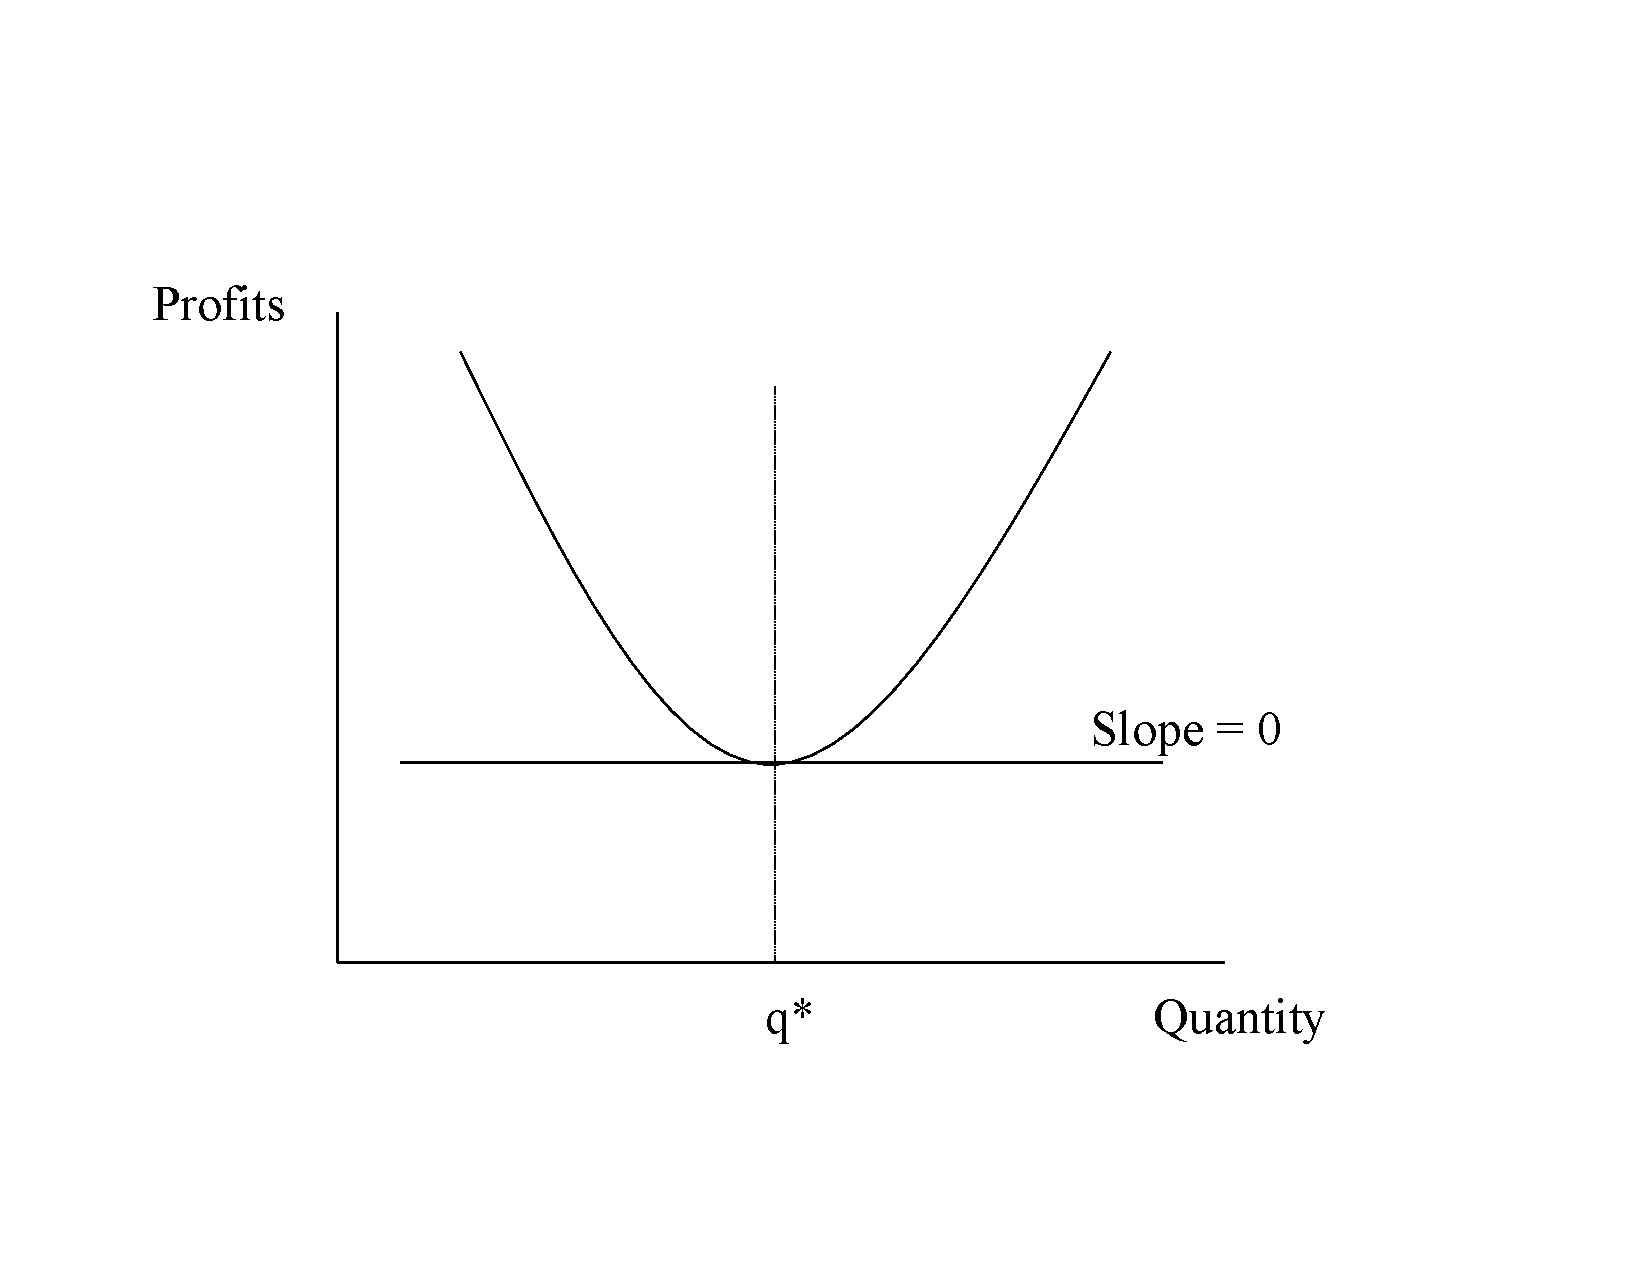
\includegraphics[scale=0.6]{math2.pdf}


\begin{eqnarray*}
\left. \frac{\partial \pi }{\partial q}\right| _{q^{\ast }}&=&0 \\
\end{eqnarray*}

but $q^{\ast }$ is a profit minimum.

We have to look at second order condition (SOC):

\begin{eqnarray*}
\left. \frac{\partial ^{2}\pi }{\left( \partial q\right) ^{2}}\right|
_{q^{\ast }}&<&0 \\
-2&<&0
\end{eqnarray*}

This guarantees that $q^{\ast }$ is a local maximum.

This method doesn't help when the function is not well behaved.

Examples:

\bigskip
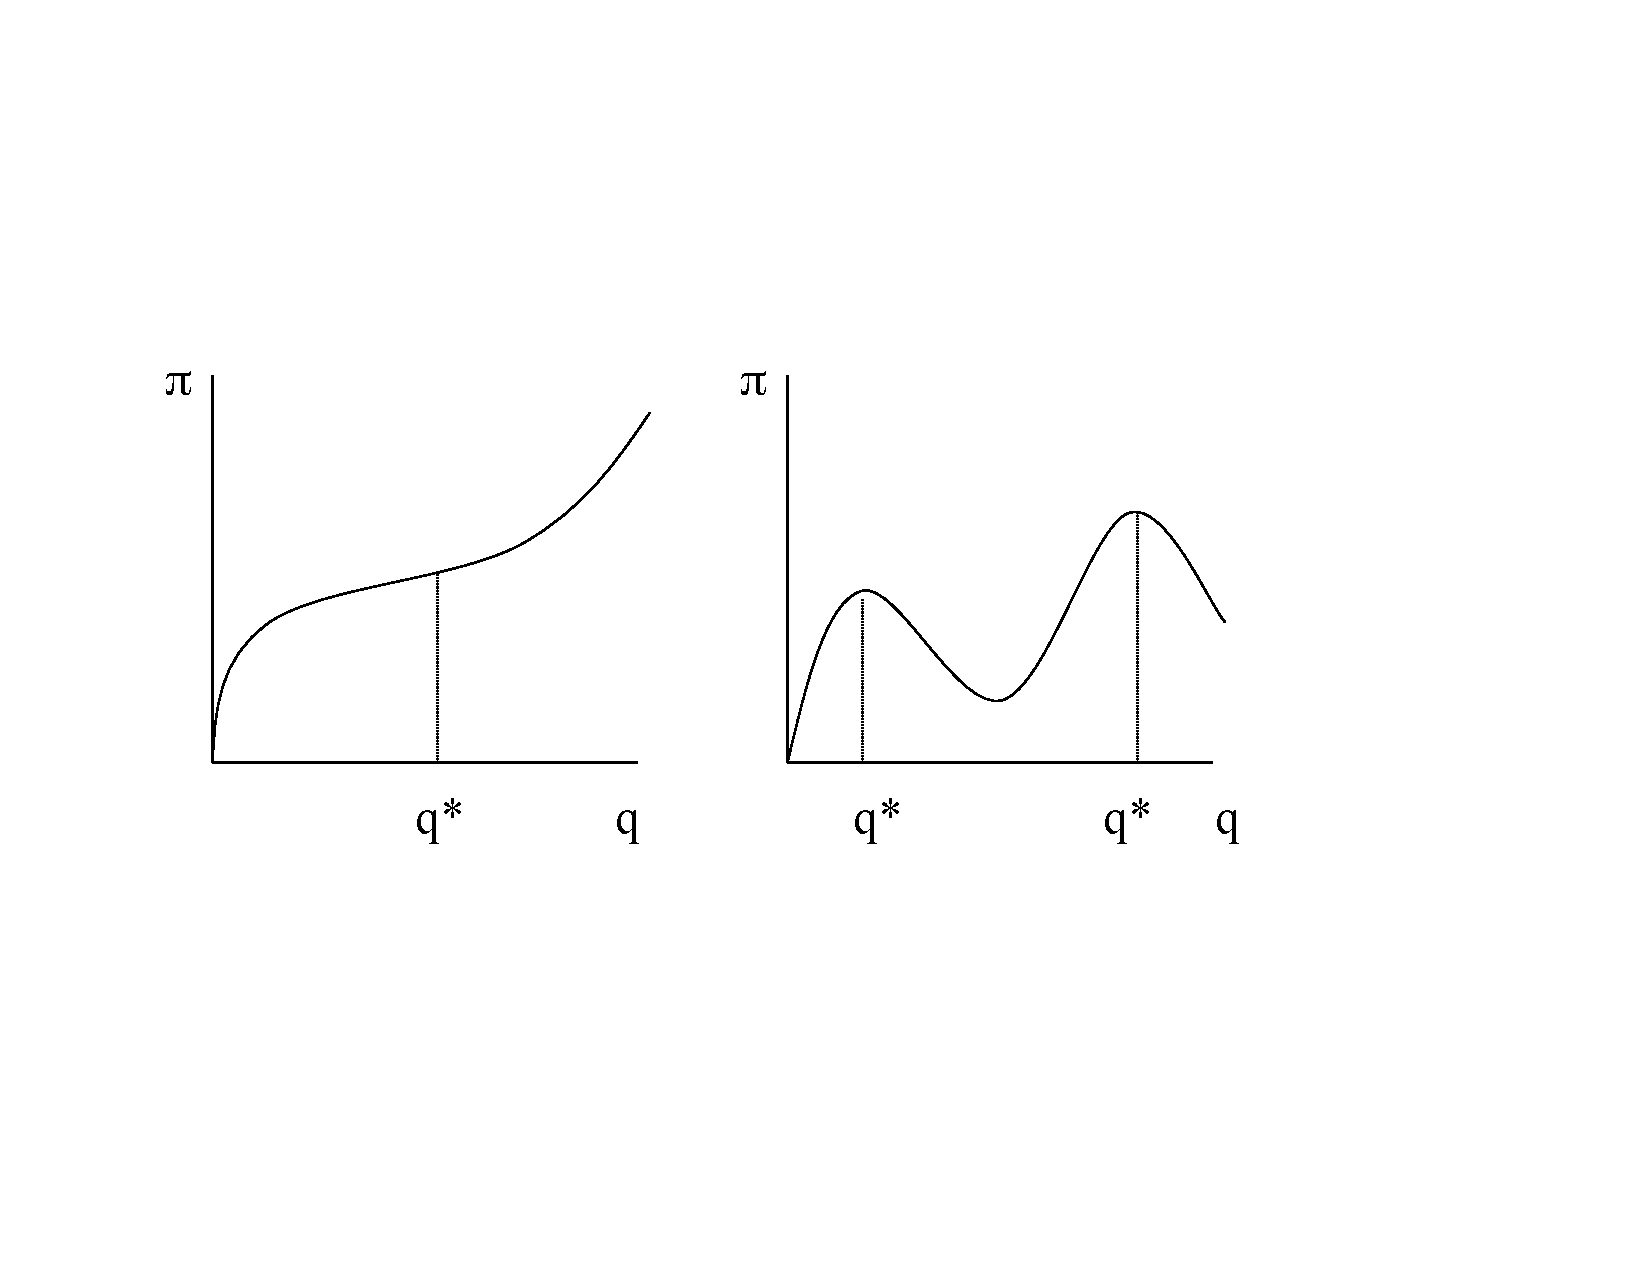
\includegraphics[scale=0.7]{math3.pdf}


We'll generally work with ``well-behaved'' \
functions: continuous, differentiable, concave. Hence we will typically not focus on
SOC. 

\bigskip

\section{Multivariate Optimization}

Given a function: 
\begin{equation*}
y=f(x_{1},x_{2},...,x_{n})
\end{equation*}

and given all partial derivatives: 
\begin{equation*}
\frac{\partial f}{\partial x_{1}}\equiv f_{1},\;\;\frac{\partial f}{\partial
x_{2}}\equiv f_{2},\;...,\;\frac{\partial f}{\partial x_{n}}\equiv f_{n}\;
\end{equation*}

First order condition (FOC) for maximum (or minimum):

\begin{equation*}
f_{1}=f_{2}=...=f_{n}=0
\end{equation*}

For multivariable functions the sufficient conditions for a critical point to be a minimum or a maximum turn out to be whether the Hessian matrix is positive definite or negative definite (all negative or all positive eigenvalues). Fortunately, we won't worry about this much and when we do it'll be in a case with two variables in which case there's a shortcut  

The Second Order Condition (SOC) for a maximum when there is more than one
variable has the following form:

\begin{eqnarray*}
f_{11} &<&0 \\
f_{11}f_{22}-(f_{12})^{2} &>&0
\end{eqnarray*}

Note that $f_{22}<0$ is implied by the above, since if $f_{11}$ and $f_{22}$
have opposite signs there is no way to get $f_{11}f_{22}-(f_{12})^{2}>0$.
Also note that it is not sufficient to have just  $f_{11}<0$ and $f_{22}<0$.

\bigskip 

For a minimum, the SOC takes the form

\begin{eqnarray*}
f_{11} &>&0 \\
f_{11}f_{22}-(f_{12})^{2} &>&0
\end{eqnarray*}

\bigskip If $f_{11}f_{22}-(f_{12})^{2}<0$, then the point in question is
neither a minimum nor a maximum.



\subsection{Concave Functions}

To simplify this we will often work with concave functions because they have the nice property that the FOC is sufficient for a global max.

\begin{definition}
A concave function is a function that always lies below any hyperplane that
is tangent to it.
\end{definition}

For example a function of one variable is concave if it always lies below
any line tangent to it.

\begin{equation*}
-1000x^2-1000y^2-xy+200
\end{equation*}

\begin{center}
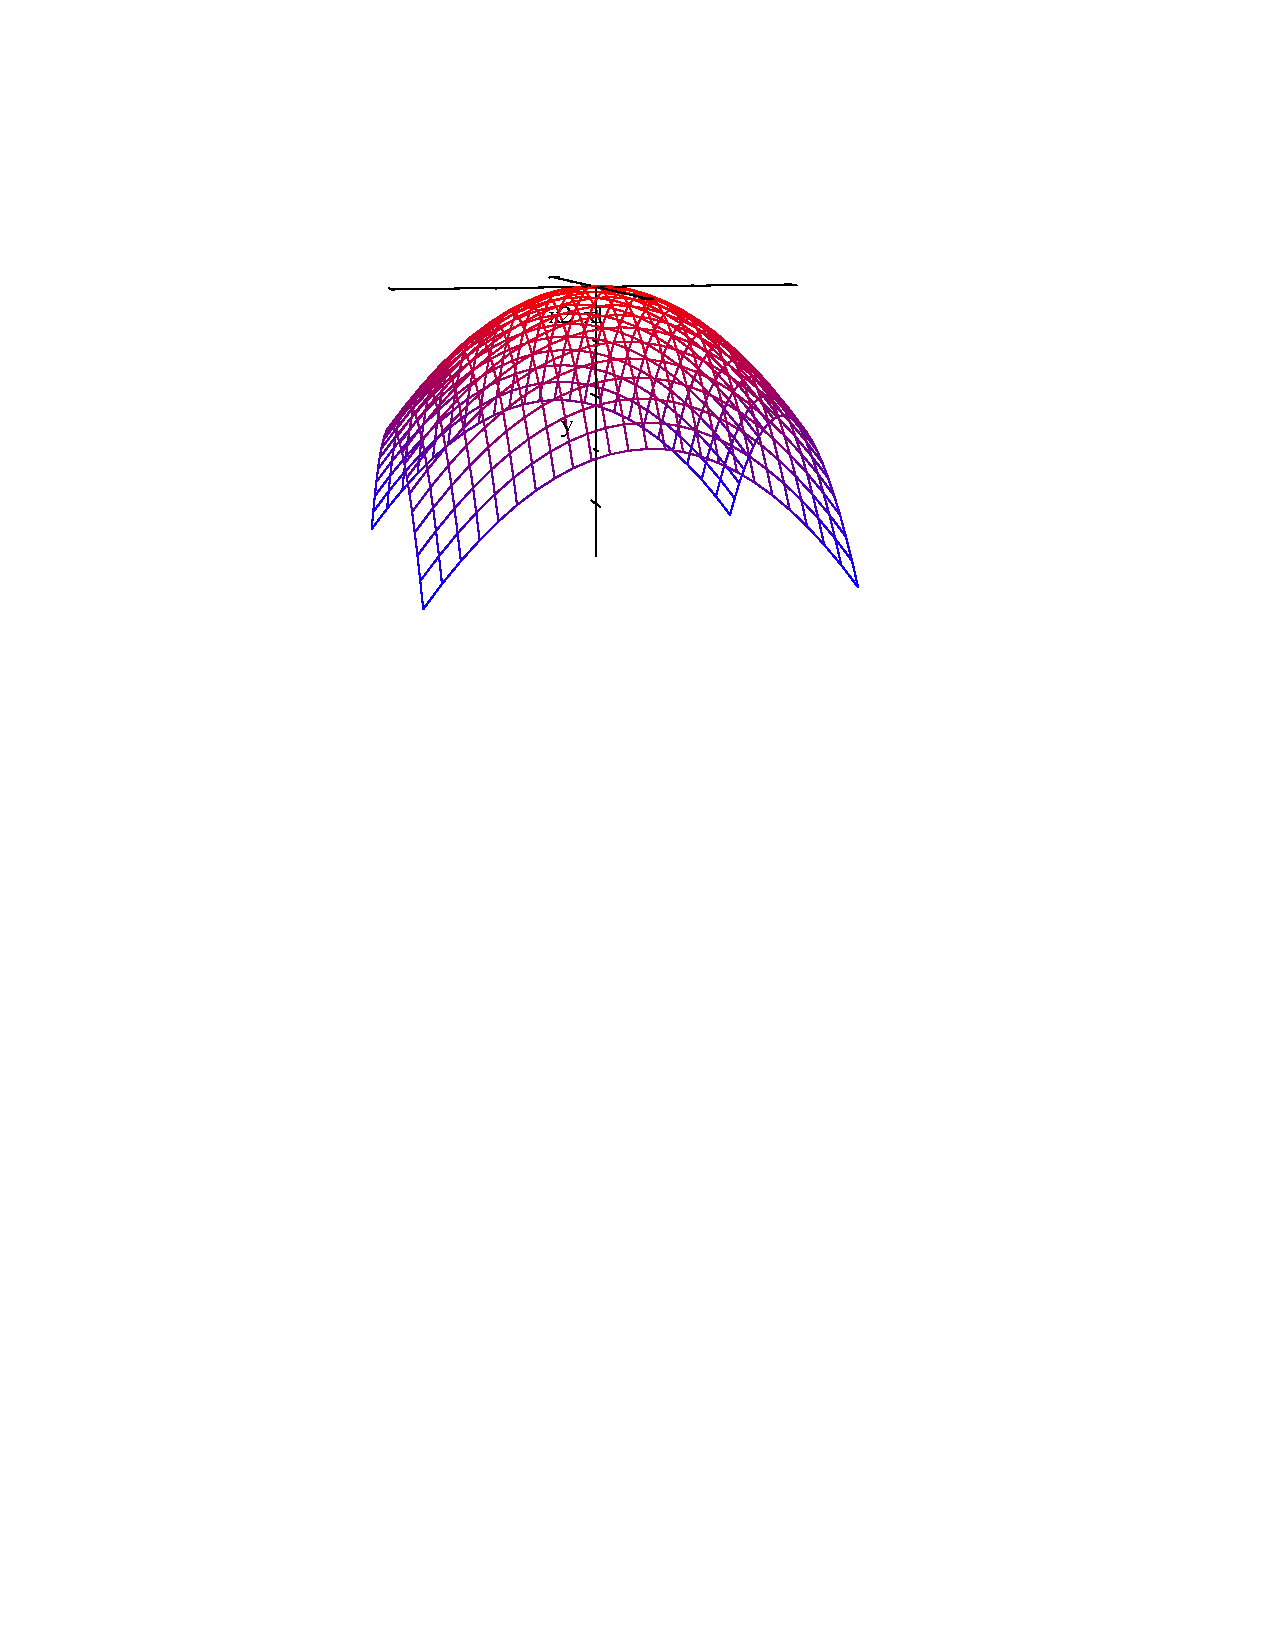
\includegraphics[scale=0.8]{math4.pdf}

Another useful definition for concave functions is that for any two points $a,b$ and $\alpha\in(0,1)$ $f(\alpha a+(1-\alpha)b)\geq \alpha f(a)+(1-\alpha)f(b)$ that is that the graph lies above any line that connects the two. You might remember from 14.01 that this implies risk aversion.


\end{center}


This set of functions satisfies the condition for concavity:

\begin{center}
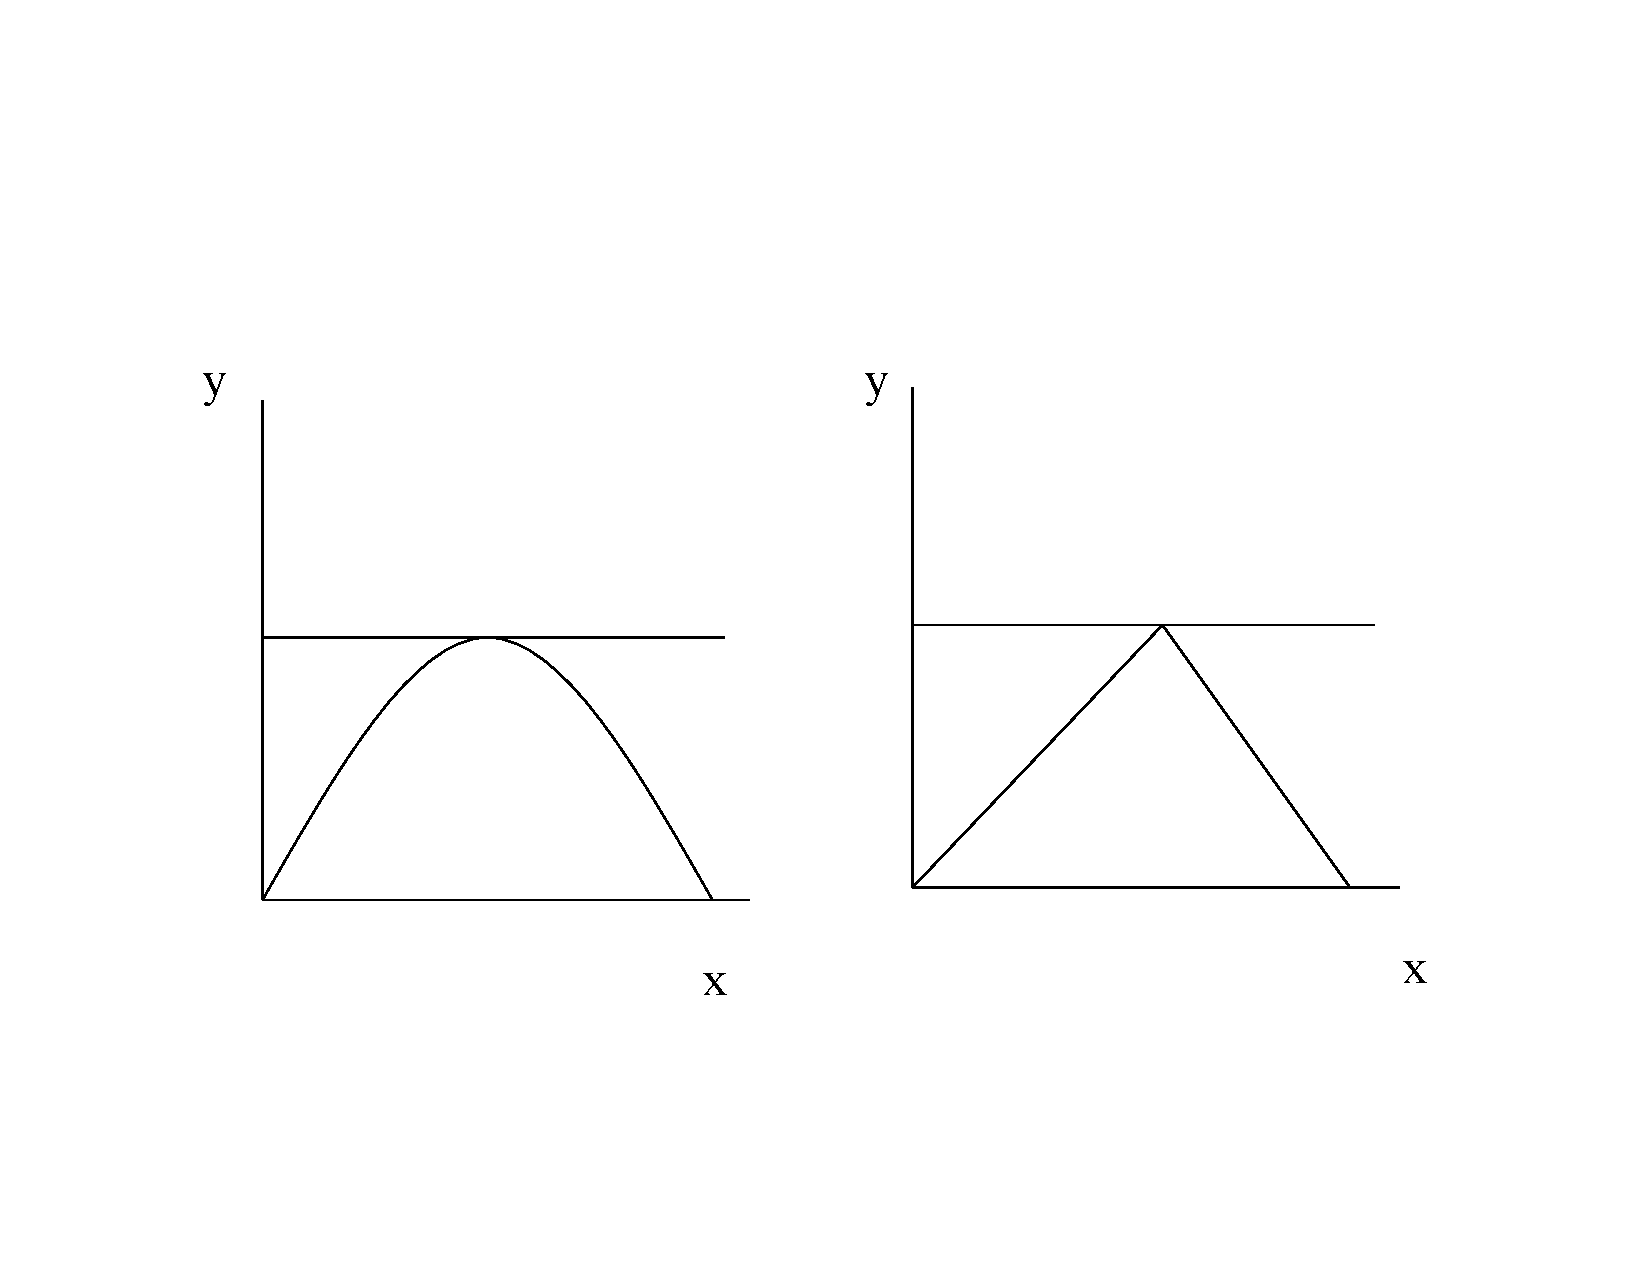
\includegraphics[scale=0.6]{math5.pdf}

This set of functions doesn't satisfy the condition for concavity:

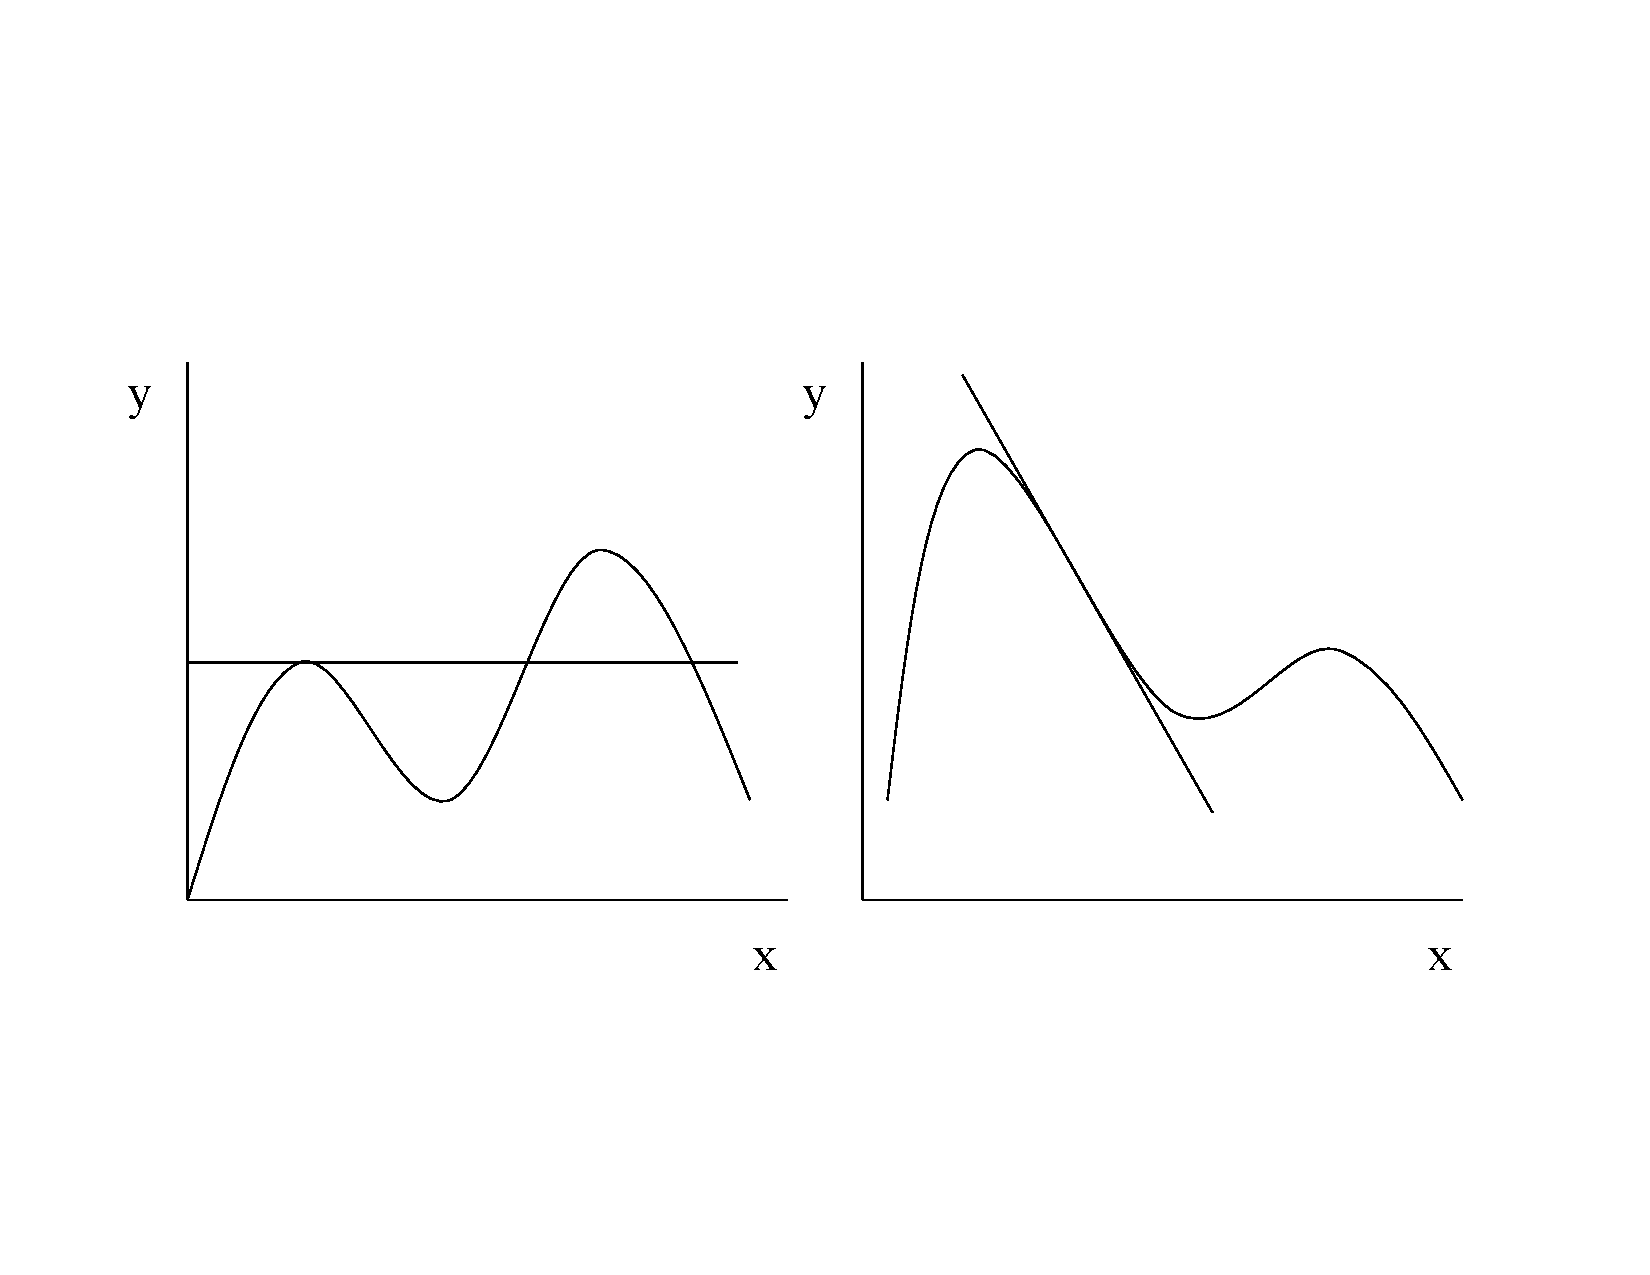
\includegraphics[scale=0.6]{math6.pdf}

\end{center}

\bigskip



\subsection{Example}

For example, now suppose we need both capital and labor to produce a good so our profit function becomes $\pi(l,k)=\ln(l)+\ln(k)-wl-rk$. We set both derivatives to zero:
\begin{eqnarray*}
\frac{\partial \pi}{\partial l}& = &0 \implies \frac{1}{l}-w=0 \\
l^*& = &\frac{1}{w} \\
\frac{\partial \pi}{\partial k}& = &0 \implies \frac{1}{k}-r=0 \\
k^*& = &\frac{1}{r}
\end{eqnarray*}

And we can check our two variable conditions:
\begin{eqnarray*}
\begin{bmatrix}
-\frac{1}{l^2} & 0 \\
0 & -\frac{1}{k^2}
\end{bmatrix} \implies f_{xx}<0 \mbox{ and } f_{xx}f_{yy}-f_{xy}^2>0
\end{eqnarray*}

Or we can note that $\pi(l,k)$ is concave and thus the FOC are sufficient.
\bigskip

We often don't want to just know what the max is. We often want to know the how changes in one variable around the maximum affect the other optimized values (comparative statics). The implicit function theorem and the envelope theorem help us with this.


\section{Implicit Functions}

Many times in economics we end up with implicit functions where exogenous
and endogenous variables are all mixed together but we still want to know how the change in one variable (say $x$) affects another say ($y$). If we could solve for$y^*(a)$ explicitly we could just differentiate and we'd be fine, but the fact that they're all mixed up means we sometimes can't solve explicitly for $y^*$. However, the derivative $\frac{\partial y}{\partial x}$ may still exist. The implicit function theorem helps us find \emph{IF it exists}.

\bigskip

Functions can be written in their implicit form or in their explicit form.

Examples:

\begin{enumerate}
\item $\;y=mx+b\;\;\;\;\;\;\;\;\;\;\;$Explicit

\item $\;y-mx-b=0\;\;\;\;\;\;\;$Implicit

\item $\;f(y,x;m,b)=0\;\;\;\;\;\;\ $Implicit
\end{enumerate}

\bigskip

Functions 2 and 3 are called implicit because the relationship between the
variables is implicitly present rather than explicitly shown as $y=f(x)$. One common source of implicit functions are first order conditions.



It's easy to work with implicit functions.%
\begin{eqnarray*}
f(x,y) &=&0\; \\
f(x,y(x)) &=&0 \\
f_{x}dx+f_{y}dy &=&0 \\
\frac{dy}{dx} &=&-\frac{f_{x}}{f_{y}}
\end{eqnarray*}

Caveat: $\frac{dy}{dx}$ may not exist...

\bigskip

\subsection{Example}

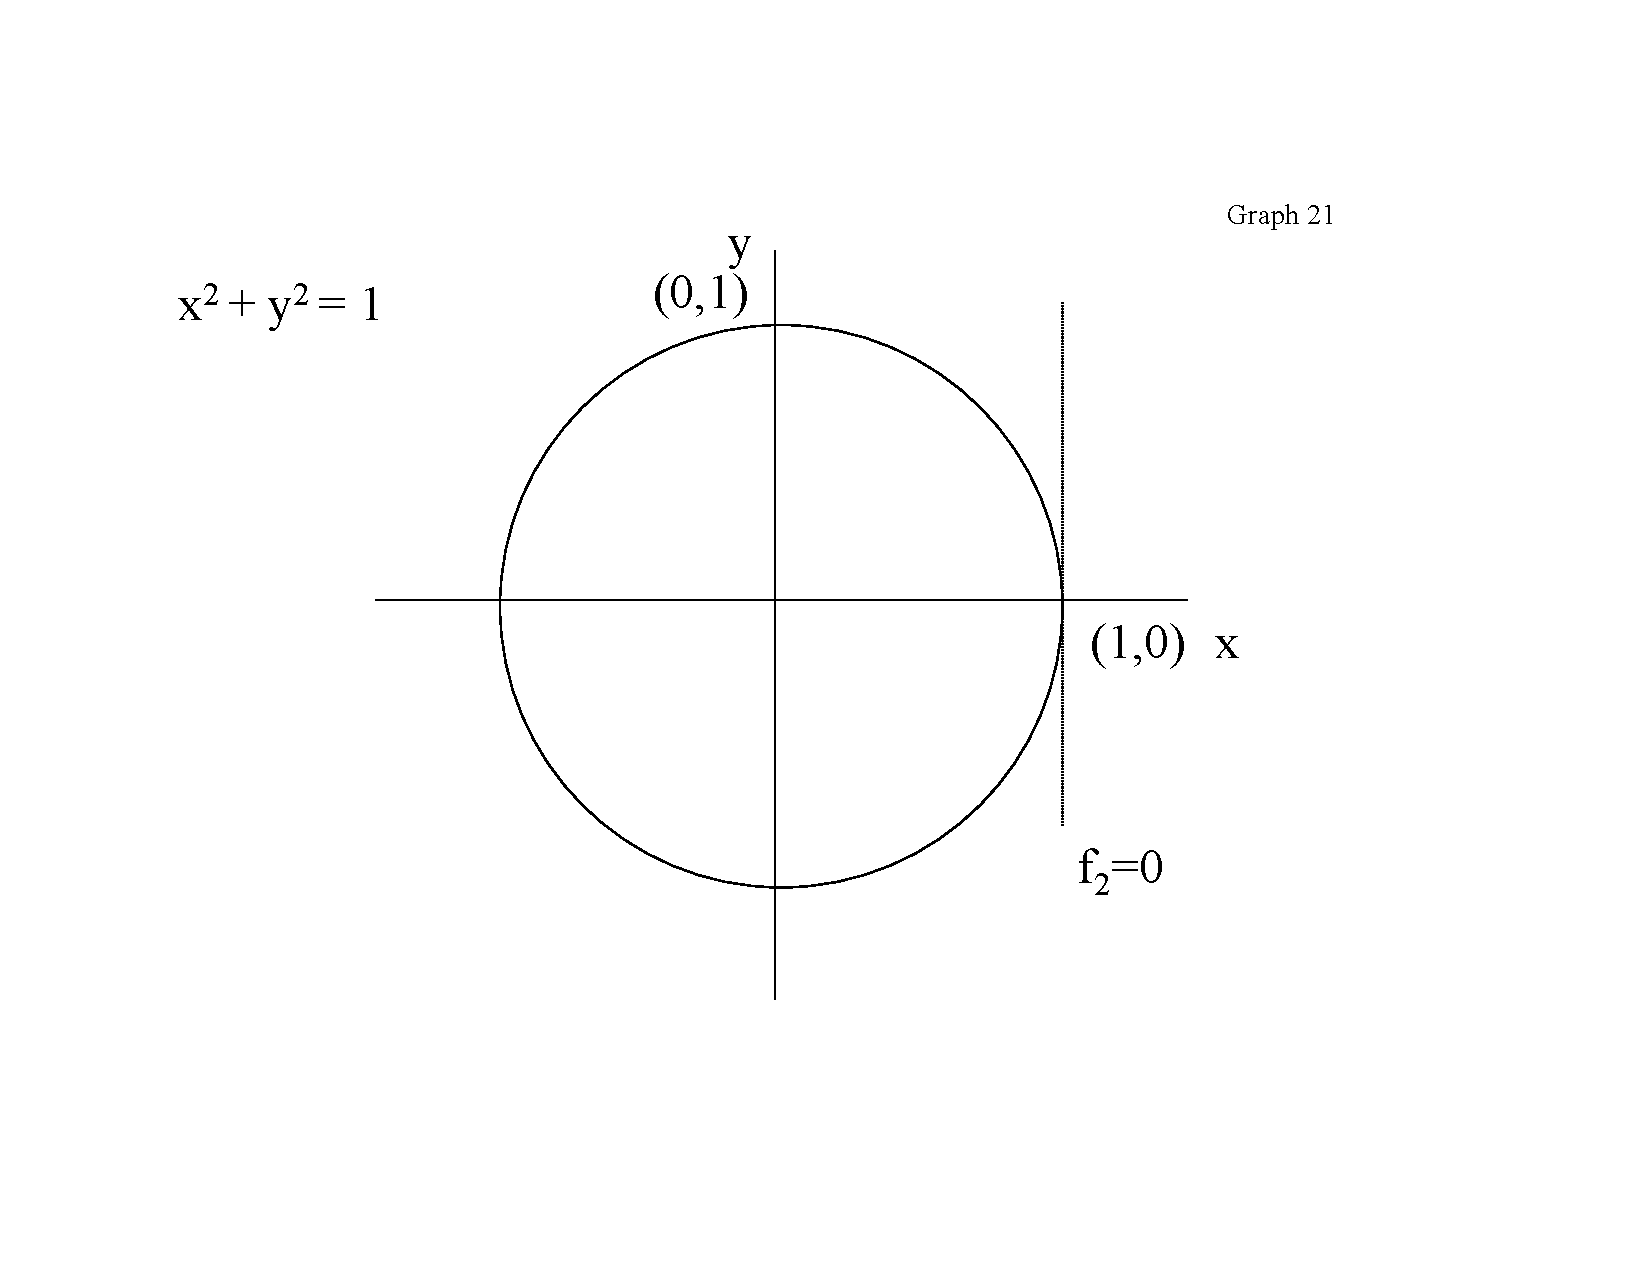
\includegraphics[scale=0.6]{math7.pdf}


\bigskip

We can write the equation for this function as follows: 
\begin{equation*}
f(x^{\ast },y(x^{\ast }))=0
\end{equation*}

which yield the following equation:

\begin{equation*}
x^{2}+y^{2}-1=0
\end{equation*}

We can differentiate and find the derivative: 
\begin{eqnarray*}
2xdx+2ydy &=&0 \\
\frac{dy}{dx} &=&-\frac{f_{1}}{f_{2}}=-\frac{x}{y}
\end{eqnarray*}

This derivative is not defined when $y=0$.

\bigskip

Q: What is the intuition for the non-existence of $\frac{dy}{dx}$ at $\
(x,y)=(1,0)$?

A: $\frac{dy}{dx}$ could be positive or negative here. Undefined.

You can see how this works formally.

Suppose there is a continuous solution $y=y(x)$ for the equation $%
F(x,y)=c\;\Rightarrow \;$ $F(x,y(x))=c$

We want to know $\frac{\partial y}{\partial x}$ for some $(x_{0},y(x_{0}))$.

Use the chain rule to differentiate.

\begin{eqnarray*}
\frac{dF(x_{0},y(x_{0}))}{dx} &=&\frac{\partial F(x_{0},y(x_{0}))}{\partial x%
}\frac{dx}{dx}+\frac{\partial F(x_{0},y(x_{0}))}{\partial y}\frac{dy(x_{0})}{%
dx}=0 \\
0 &=&\frac{\partial F(x_{0},y(x_{0}))}{\partial x}+\frac{\partial
F(x_{0},y(x_{0}))}{\partial y}y^{\prime }(x_{0}) \\
y^{\prime }(x_{0}) &=&-\frac{\frac{\partial F(x_{0},y(x_{0}))}{\partial x}}{%
\frac{\partial F(x_{0},y(x_{0}))}{\partial y}}
\end{eqnarray*}

Necessary condition for $y^{\prime }(x_{0})$ to exist is that $\frac{%
\partial F(x_{0},y(x_{0}))}{\partial y}\neq 0$ (Implicit function theorem)

It turns out that this is sufficient also.

In the multivariate case this condition can be written as $\frac{\partial
F(x_{1}^{\ast },...,x_{n}^{\ast },y^{\ast })}{\partial y}\neq 0$

\subsection{Example}

Given the following function: 
\begin{eqnarray*}
2x^{2}+y^{2} &=&225, \\
y &\geq &0
\end{eqnarray*}

we want to find $\frac{dy}{dx}.$

\bigskip

\begin{enumerate}
\item One way to find the derivative we are looking for is to find $y$ as a
function of $x$%
\begin{eqnarray*}
y &=&\sqrt{225-2x^{2}} \\
\frac{dy}{dx} &=&\frac{1}{2}\left( 225-2x^{2}\right) ^{-\frac{1}{2}}(-4x)= \\
&=&\frac{-4x}{2\sqrt{225-2x^{2}}}=-\frac{2x}{y}
\end{eqnarray*}

\item The other way to find it is to use the implicit function method:
\end{enumerate}

\begin{itemize}
\item Write: $2x^{2}+y^{2}-225=0$

\item Find the total differential: $4xdx+2ydy=0$

\item Rearrange: 
\begin{equation*}
\frac{dy}{dx}=-\frac{2x}{y}
\end{equation*}
\end{itemize}

\subsection{Example}

Take a more complicated example: 
\begin{equation*}
g(x,y)=x^{2}-3xy+y^{3}-7=0
\end{equation*}

What is $\left. \frac{dy}{dx}\right| _{x=4,y=3}$?

In this case making use of the implicit function theorem is the only way to
find the derivative we are interested in.

\begin{enumerate}
\item Find total differential:

\begin{eqnarray*}
2xdx-3ydx-3xdy+3y^{2}dy &=&0 \\
3y^{2}dy-3xdy &=&-2xdx+3ydx \\
\frac{dy}{dx} &=&\frac{3y-2x}{3y^{2}-3x}=-\frac{g_x(x,y)}{g_y(x,y)}
\end{eqnarray*}

\item To find the derivative at the point we simply substitute:

\begin{equation*}
\left. \frac{dy}{dx}\right| _{x=4,y=3}=\frac{9-8}{27-12}=\frac{1}{15}
\end{equation*}

\item What is $y$ at $x=4.3$?

We can approximate it by: 
\begin{eqnarray*}
&&y(4)+\left. \frac{dy}{dx}\right| _{x=4}(0.3) \\
y(4.3) &\approx &3+0.3\times \frac{1}{15}=3.02
\end{eqnarray*}

If we solve numerically for $y$ at $x=4.3$ we get $3.01475$.
\end{enumerate}

\bigskip

\subsection{Applications of Implicit Functions}

Being able to handle implicit functions turns out to be useful when one
deals with utility functions and indifference curves.

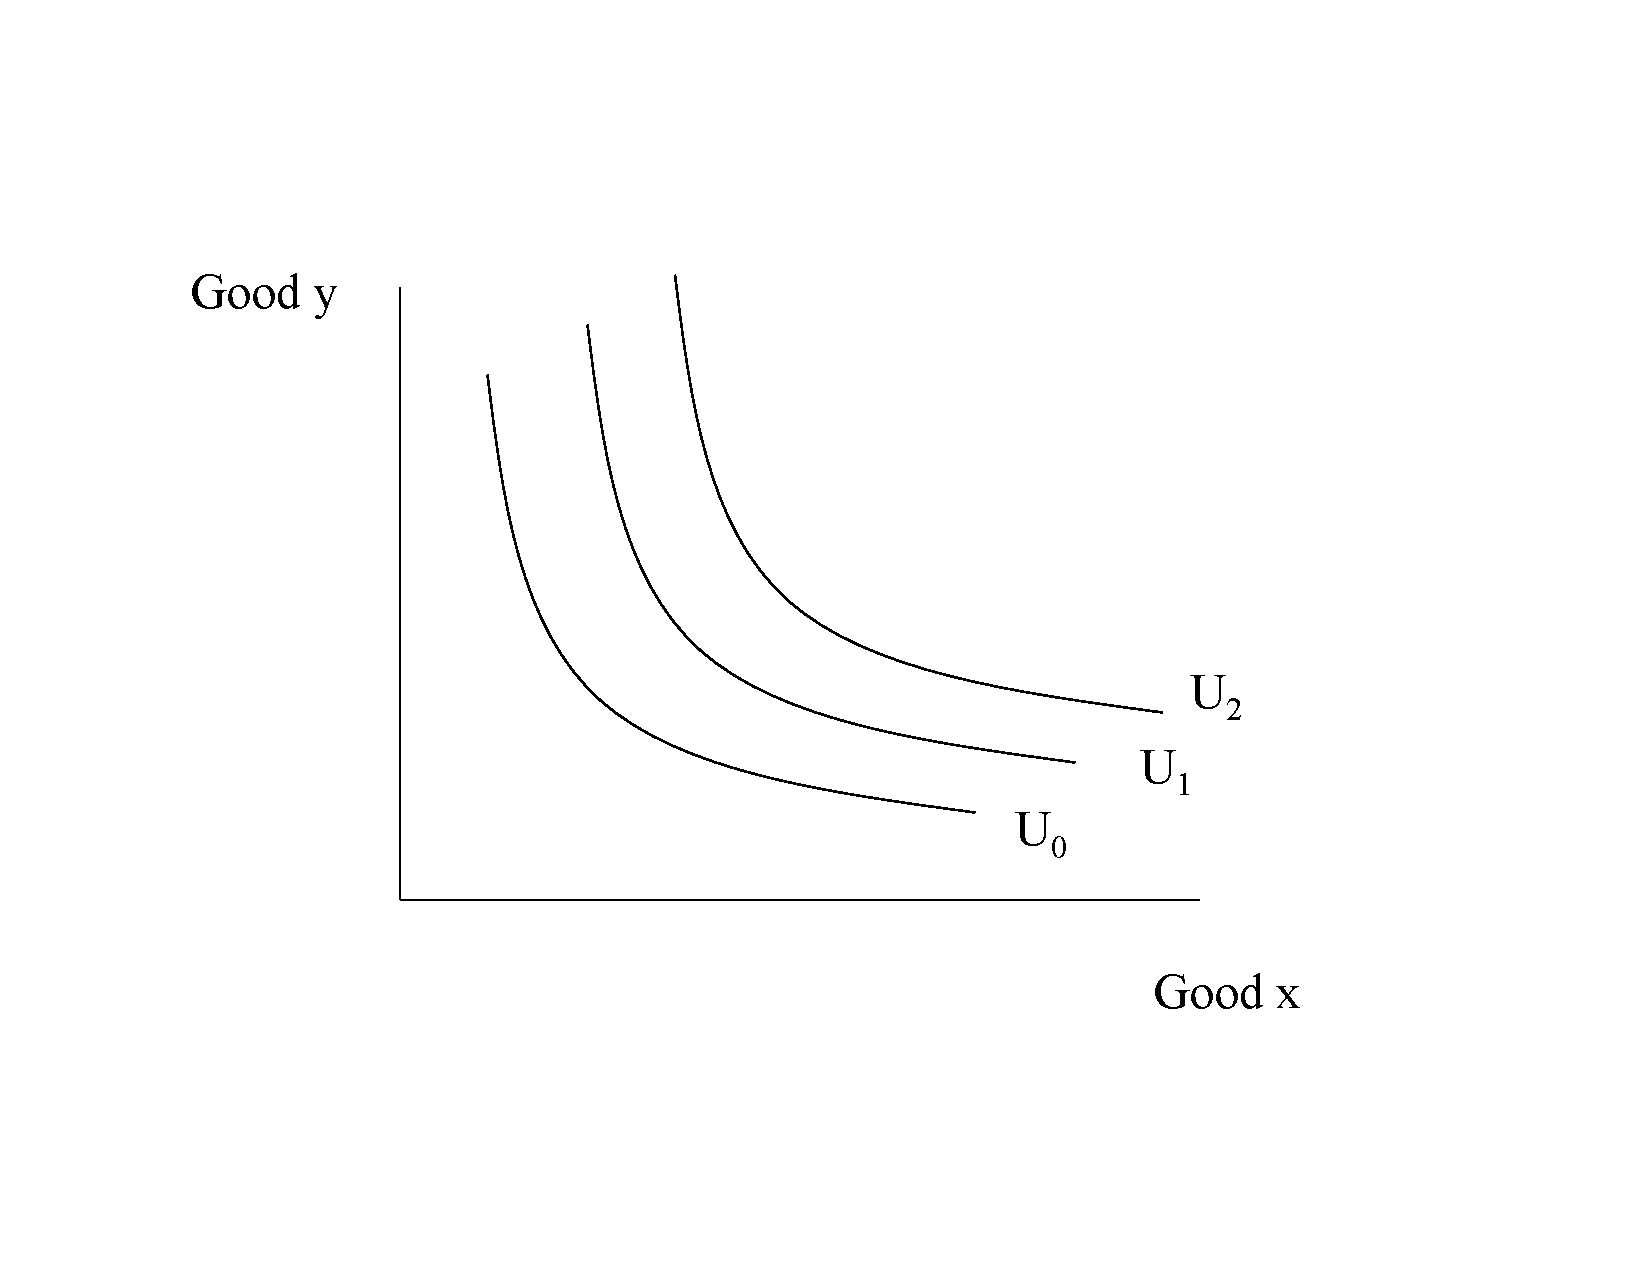
\includegraphics[scale=0.6]{math8.pdf}


Along an indifference curve, we have $U(x,y)=\overline{U}$

The implicit function $U(x^{\ast },y^{\ast }(x^{\ast }))=\overline{U}$ $\ $%
tells how much $y$ we'd give up for a little more $x$ (at the margin) while
holding total utility constant. 
\begin{eqnarray*}
U(x^{\ast },y^{\ast }(x^{\ast })) &=&\overline{U} \\
\frac{\partial U}{\partial x}dx+\frac{\partial U}{\partial y}dy &=&0 \\
\frac{dy}{dx} &=&-\frac{U^{\prime }(x)}{U^{\prime }(y)}
\end{eqnarray*}

\bigskip

\section{Envelope Theorems}

\bigskip

A shortcut for taking derivatives of optimized functions with respect to
their parameters.

\begin{theorem}
(Envelope Theorem for the unconstrained case). Let $f(x,a)$ be a $C^{1}$
function of $x\in R^{n}$ and the scalar $a$. For each $a$ consider the
unconstrained maximization: 
\begin{equation*}
\max \;f(x;a)\;w.r.t.\;x
\end{equation*}%
Let $x^{\ast }\left( a\right) $ be a solution of this problem. Suppose that $%
x^{\ast }(a)$ is a $C^{1}$ function of $\ a$. Then, 
\begin{equation*}
\underset{Total\;derivative}{\frac{d}{da}f(x^{\ast }(a),a)}=\underset{%
Partial\;derivative}{\frac{\partial }{\partial a}f(x^{\ast }(a),a)}
\end{equation*}
\end{theorem}

\bigskip

\begin{proof}
\begin{eqnarray*}
\frac{d}{da}f(x^{\ast }(a),a) &=&\underset{=0}{\underbrace{\sum \frac{%
\partial f}{\partial x_{i}}(x^{\ast }(a),a)\frac{\partial x_{i}^{\ast }(a)}{%
\partial a}}}+\frac{\partial f}{\partial a}(x^{\ast }(a),a)= \\
&=&\frac{\partial f}{\partial a}(x^{\ast }(a),a)
\end{eqnarray*}%
where the first term of the derivative is zero because: 
\begin{equation*}
\frac{\partial f}{\partial x_{i}}(x^{\ast }(a),a)=0\;\;\forall i=1,2,...,n\;
\end{equation*}%
These are the FOC\ of the maximization problem to obtain $x^{\ast }$.
\end{proof}

Note: much more intuitive - \underline{and useful} than it looks

\textbf{Example:}

Take the following function 
\begin{equation*}
y=-x^{2}+ax
\end{equation*}%
We want to know $\frac{dy^{\ast }}{da}$ where $y^{\ast }$ is the maximized
value of the above function. We can proceed in the two ways:

\begin{enumerate}
\item \bigskip Find $x^{\ast }$ through single variable optimization and
then substitute.%
\begin{eqnarray*}
\frac{dy}{dx} &=&-2x+a=0 \\
x^{\ast } &=&\frac{a}{2} \\
y^{\ast } &=&-\left( \frac{a}{2}\right) ^{2}+a\left( \frac{a}{2}\right) =%
\frac{a^{2}}{4} \\
\frac{dy^{\ast }}{da} &=&\frac{a}{2}=x^{\ast }
\end{eqnarray*}

\item Find the derivative using the envelope theorem: 
\begin{eqnarray*}
y^{\ast } &=&-\left( x^{\ast }\right) ^{2}+ax^{\ast } \\
\left. \frac{\partial y}{\partial a}\right\vert _{x=x^{\ast }} &=&x^{\ast }=%
\frac{dy^{\ast }}{da}
\end{eqnarray*}
\end{enumerate}

\subsection{Visual Explanation of the Envelope Theorem}

\bigskip Remember that $y=-x^{2}+ax$ and $y^{\ast }=f(a,x^{\ast }(a))=\frac{%
a^{2}}{4}$

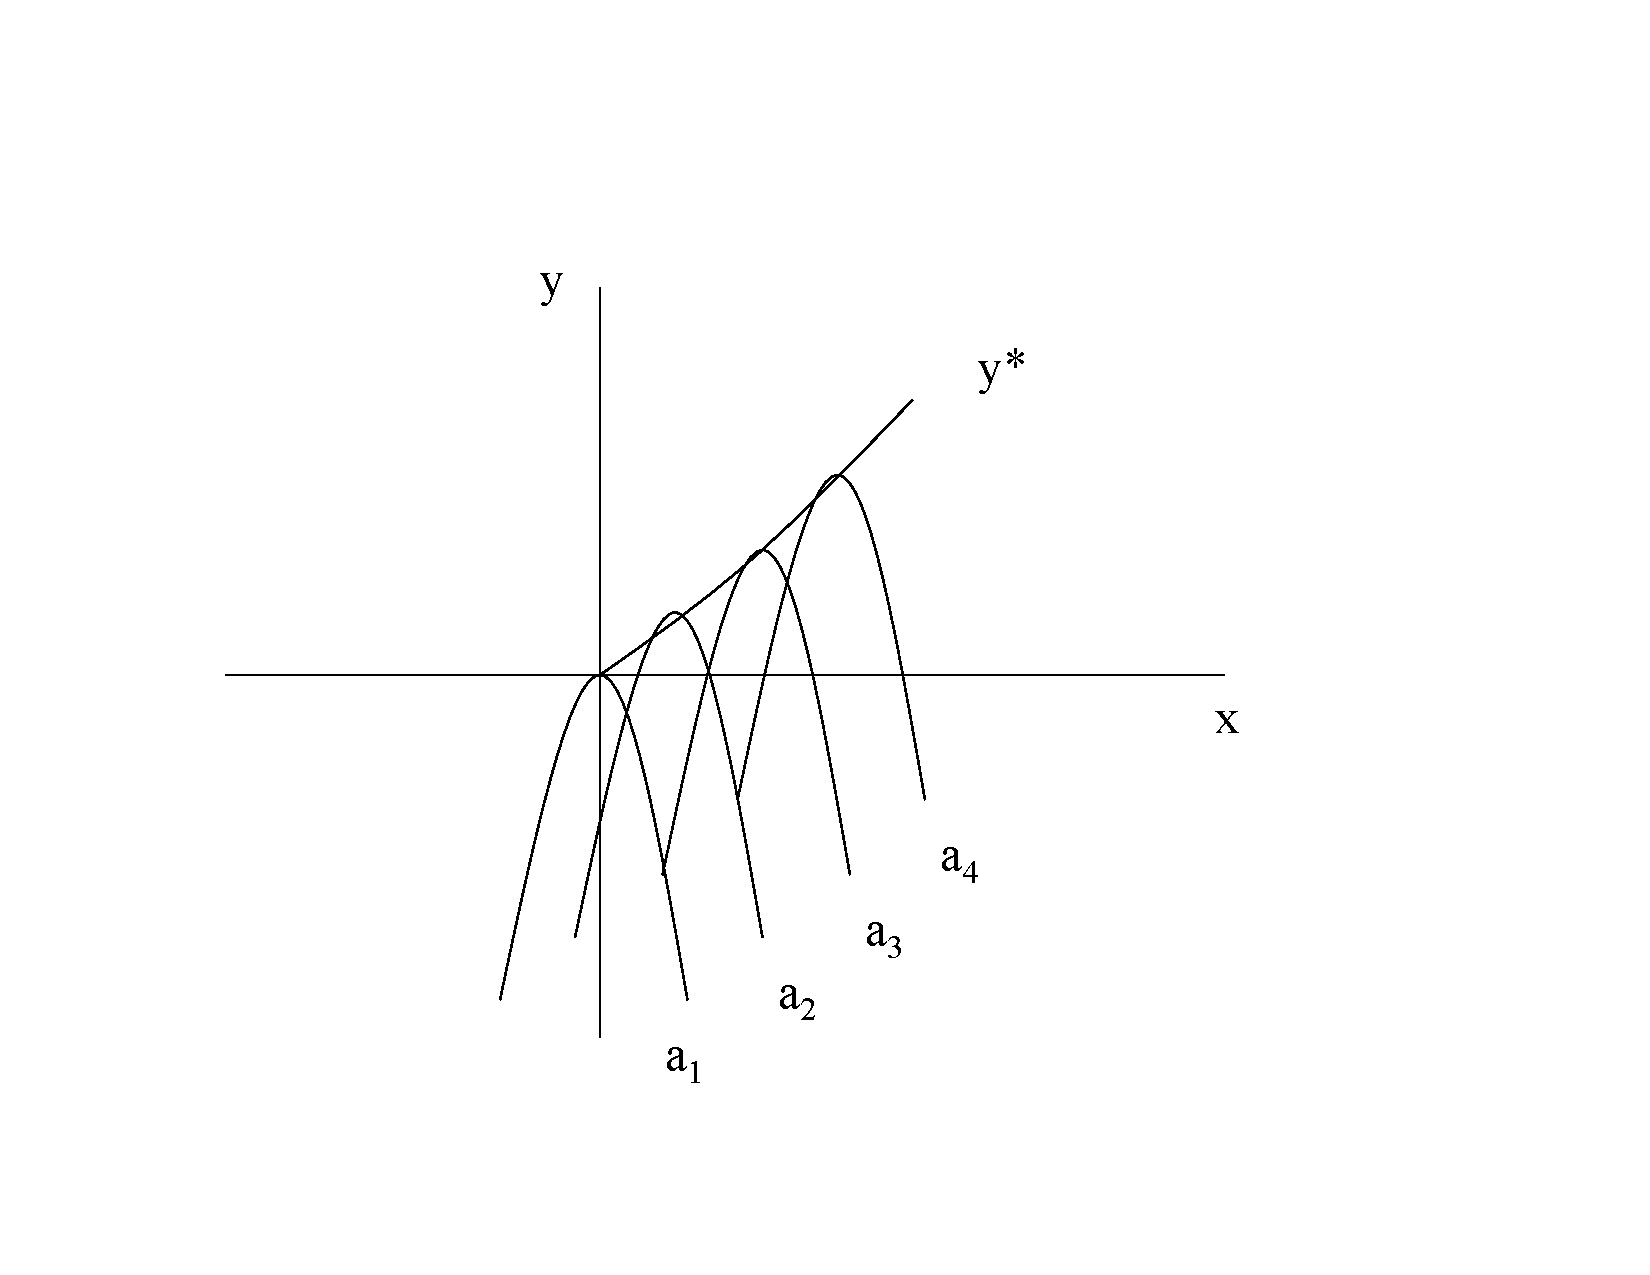
\includegraphics[scale=0.6]{math9.pdf}


Note: Envelope Theorem is a linear approximation and hence holds in an
''envelope'' surrounding $x^{\ast }(a)$.

It is called Envelope Theorem because we are evaluating the upper envelope
of a function.

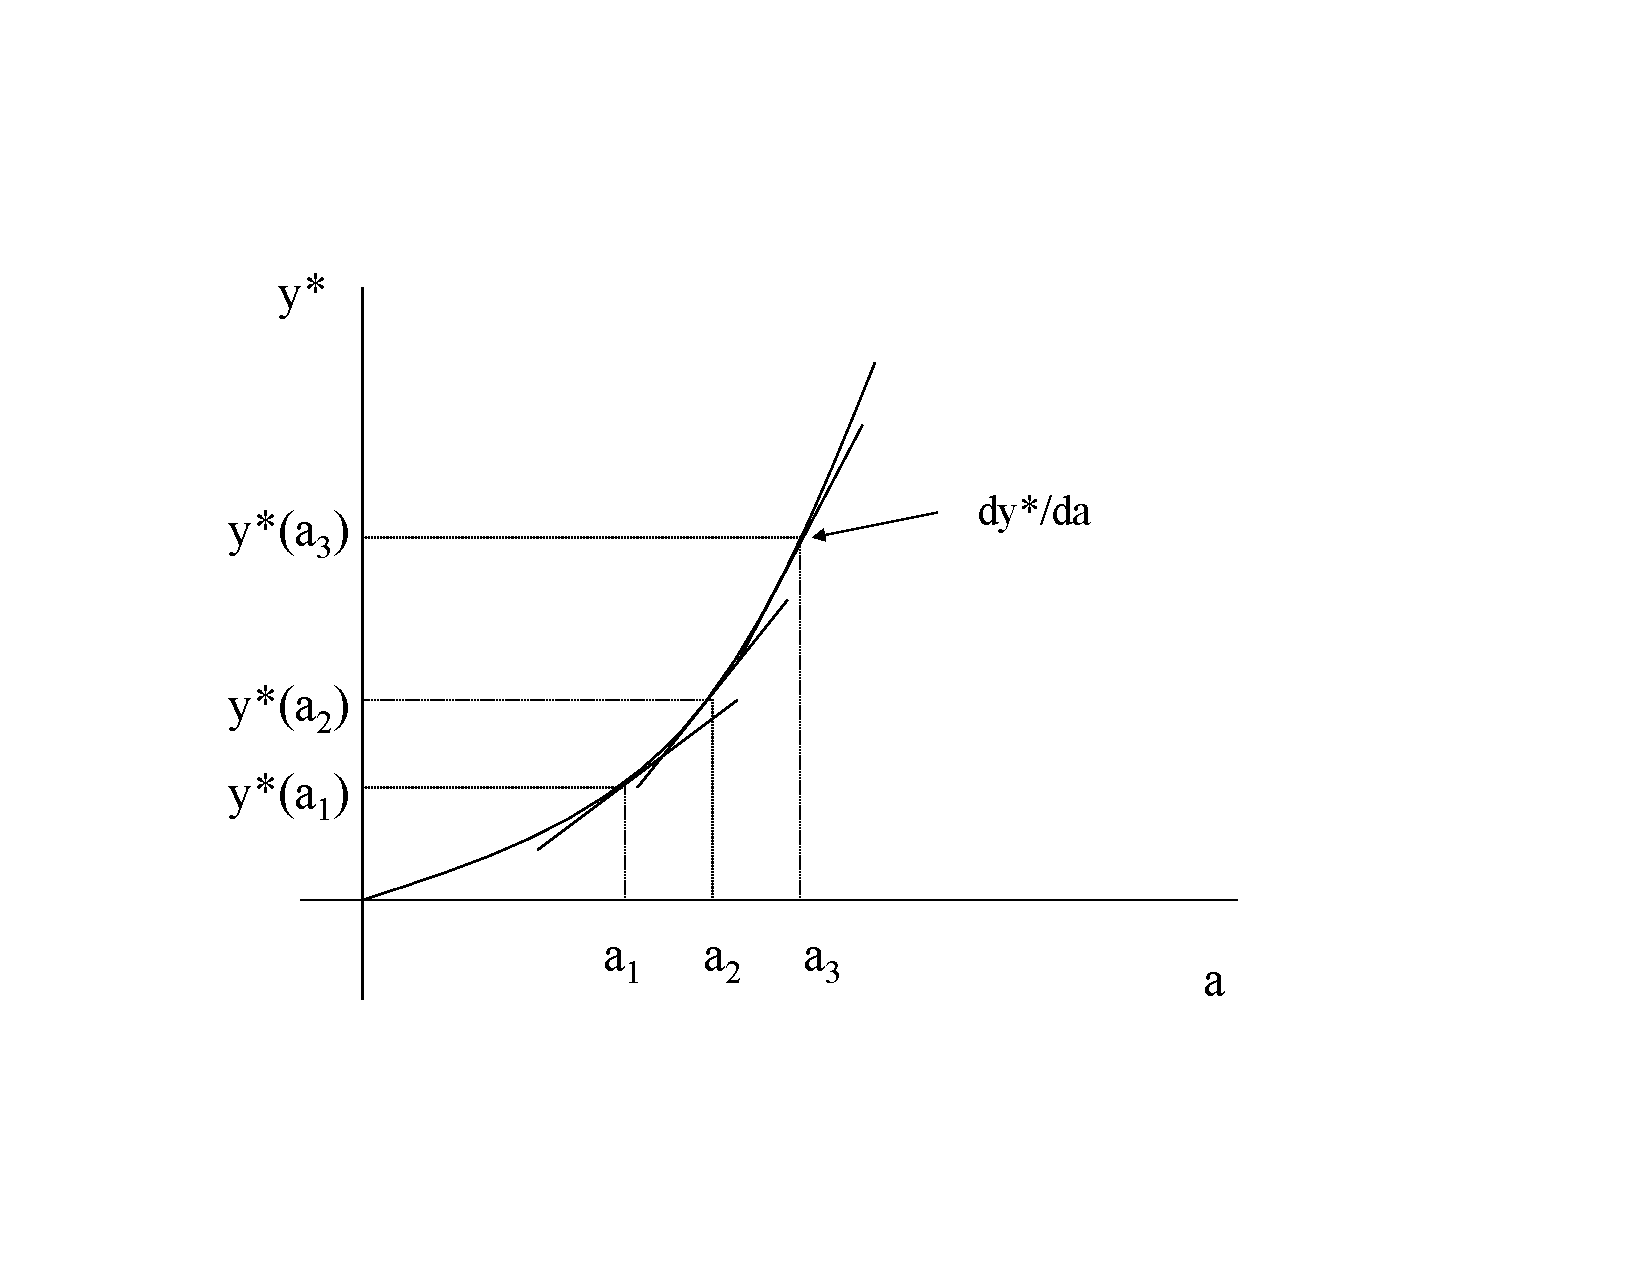
\includegraphics[scale=0.6]{math10.pdf}


\bigskip

The function drawn in this graph is such that its derivative at each point is

\begin{equation*}
\frac{\partial y^{\ast }}{\partial a}=x^{\ast }(a)
\end{equation*}

\begin{center}
\bigskip
\end{center}

\textit{Remember: }Envelope Theorem is multi-variate

\begin{eqnarray*}
y^{\ast } &=&f\left[ x_{1}^{\ast }(a),x_{2}^{\ast }(a),...,x_{n}^{\ast }(a);a%
\right] \\
\frac{dy^{\ast }}{da} &=&\underset{=0}{\underbrace{\frac{\partial f}{%
\partial x_{1}}\frac{\partial x_{1}}{\partial a}+...+\frac{\partial f}{%
\partial x_{n}}\frac{\partial x_{n}}{\partial a}}}+\frac{\partial f}{%
\partial a} \\
\frac{dy^{\ast }}{da} &=&\frac{\partial f}{\partial a}
\end{eqnarray*}

\bigskip

\section{Constrained Maximization}

Most maximization problems in economics are subject to constraints\textbf{:}

\begin{itemize}
\item maximize utility subject to budget constraint

\item maximize social welfare subject to a resource constraint

\item maximize profits subject to a technological constraint
\end{itemize}

The tool for maximizing constrained functions is the Lagrangian Method.

This a ``trick" that turns out to have very useful economic content.

\bigskip

\subsection{Lagrangian Method}

\bigskip

\textit{Problem:}

\begin{eqnarray*}
\max \;y &=&f(x_{1},x_{2},...,x_{n}) \\
s.t.\;g(x_{1},x_{2},...,x_{n}) &=&0
\end{eqnarray*}

\textit{Setup:}

\begin{equation*}
\mathcal{L} =f(x_{1},x_{2},...,x_{n})+\lambda g(x_{1},x_{2},...,x_{n})
\end{equation*}

FOC's 
\begin{eqnarray*}
\frac{\partial \mathcal{L} }{\partial x_{1}} &=&f_{1}+\lambda g_{1}=0 \\
&&... \\
\frac{\partial \mathcal{L} }{\partial x_{n}} &=&f_{n}+\lambda g_{n}=0 \\
\frac{\partial \mathcal{L} }{\partial \lambda } &=&g=0
\end{eqnarray*}

This way we obtain as many equations as unknowns, since we introduced
another unknown, $\lambda $.

One solves simultaneously for $x_{1}^{\ast },$ $x_{2}^{\ast },...,$ $%
x_{n}^{\ast }$ and $\lambda $.

$\lambda $ has a special interpretation that we will discuss.

\bigskip

\subsection{Example: Optimal fence dimensions}

Given a fencing perimeter of length $p$ how do we maximize the fenced area
(provided that the area must have a rectangular shape)?

So the problem can be summarized as follows: 
\begin{eqnarray*}
&&\max \;xy \\
s.t.\;2x+2y &=&p
\end{eqnarray*}

The Lagrangian for this problem is: 
\begin{eqnarray*}
\mathcal{L} &=&xy+\lambda (p-2x-2y) \\
\frac{\partial \mathcal{L} }{\partial x} &=&y-2\lambda =0 \\
\frac{\partial \mathcal{L} }{\partial x} &=&x-2\lambda =0 \\
\frac{\partial \mathcal{L} }{\partial \lambda } &=&p-2x-2y=0 \\
\frac{y}{2} &=&\frac{x}{2}=\lambda \\
x &=&y=\frac{p}{4} \\
\lambda &=&\frac{p}{8}
\end{eqnarray*}

\begin{itemize}
\item We can conclude that the optimal fence is square $(x=y)$.

\item What is the interpretation of $\lambda =\frac{p}{8}$?
\end{itemize}

Observe that: 
\begin{equation*}
\frac{f_{1}}{-g_{1}}=\frac{f_{2}}{-g_{2}}=\lambda
\end{equation*}

where $f_{1}$ is the marginal gain to the lagrangian from adding one more
unit of $x$ and $g_{1}$ is the marginal cost of adding more $x$ in terms of
tightening the constraint and hence reducing feasible $y$.

This ratio, $\lambda $, is called the ``shadow price'' of the constraint.

$\lambda $ is, in other words, the opportunity cost of the constraint at the
margin expressed in units of the maximand. It is the gain in terms of
maximand obtained by relaxing the constraint by one unit.

In our example $\lambda $ tells us the increase in area we can obtain by
increasing the size of the perimeter by one unit.

$\lambda =\frac{p}{8}$ implies that relaxing the constraint that $2x+2y=p$
by one unit would allow us to increase the maximand area by $\frac{p}{8}$.

Let's check this:

Let $p=40\;\Rightarrow \,x=y=10,\;A=100$

Now let $p=41\;\Rightarrow \,x=y=10.25,\;A=105.06$ which confirms that $%
\Delta A=5.06\approx \frac{40}{8}$

The multiplier $\lambda $ is quite close to the actual change in A for a
one-unit change in the constraint (and it would be exactly correct for a
small enough change in the perimeter).


\subsection{Example}

\begin{eqnarray*}
&&\max \;U=x^{\frac{1}{2}}y^{\frac{1}{2}} \\
s.t.\;x+y &=&I \\
\mathcal{L} &=&\;x^{\frac{1}{2}}y^{\frac{1}{2}}+\lambda \left( I-x-y\right)
\\
\frac{\partial \mathcal{L} }{\partial x} &=&\frac{1}{2}x^{-\frac{1}{2}}y^{%
\frac{1}{2}}-\lambda =0 \\
\frac{\partial \mathcal{L} }{\partial y} &=&\frac{1}{2}x^{\frac{1}{2}}y^{-%
\frac{1}{2}}-\lambda =0 \\
\frac{\partial \mathcal{L} }{\partial \lambda } &=&I-x-y=0 \\
x &=&y=\frac{I}{2},\;\;\lambda =\frac{1}{2}
\end{eqnarray*}

Let's just check the multiplier's implication:

\begin{eqnarray*}
f(x,y,4) &=&2^{\frac{1}{2}}2^{\frac{1}{2}}=2 \\
f(x,y,5) &=&2.5^{\frac{1}{2}}2.5^{\frac{1}{2}}=2.5 \\
\Delta f &=&\frac{1}{2}=\lambda
\end{eqnarray*}

\subsection{Envelope Theorem for Constrained Problems}

Let $x^{\ast }(a)$ denote the solution to the following problem:

\begin{eqnarray*}
&&\max \;y=\;f(x) \\
s.t.\;g(x;a) &=&0
\end{eqnarray*}

Let $\lambda $ be the Lagrange multiplier for the constraint in this problem.

Then:

\begin{equation*}
\underset{%
\begin{array}{c}
Total\;derivative\;of\; \\ 
the\;original\;function\;f%
\end{array}%
}{\underbrace{\frac{d}{da}f(x^{\ast }(a))}}=\underset{%
\begin{array}{c}
Partial\;derivative \\ 
of\;Lagrangian%
\end{array}%
}{\underbrace{\lambda \frac{\partial g(x;a)}{\partial a}=\frac{\partial }{%
\partial a}\mathcal{L} (x^{\ast }(a),\lambda (a),a)}}
\end{equation*}

Why is this true? First use the chain rule:

\begin{equation*}
\underbrace{\frac{d}{da}f(x^{\ast }(a))}=\sum_{i}\frac{\partial f(x^{\ast
}(a),a)}{\partial x_{i}}\frac{dx_{i}^{\ast }}{da}
\end{equation*}

\bigskip The FOC for maximizing the Lagrangean $\mathcal{L} \left( x,\lambda
,a\right) =f(x)+\lambda g(x;a)$ are

\begin{equation*}
\frac{\partial \mathcal{L} \left( x,\lambda ,a\right) }{\partial x_{i}}=%
\frac{\partial f\left( x\right) }{\partial x_{i}}+\lambda ^{\ast }\frac{%
\partial g}{\partial x_{i}}=0
\end{equation*}

\bigskip So%
\begin{equation*}
\frac{d}{da}f(x^{\ast }(a))=-\lambda \sum_{i}\frac{\partial g}{\partial
x_{i}}\frac{dx_{i}^{\ast }}{da}
\end{equation*}

\bigskip But by taking the derivative of $g(x;a)=0$ with respect to $a$ we
get 
\begin{equation*}
\sum_{i}\frac{\partial g}{\partial x_{i}}\frac{dx_{i}^{\ast }}{da}+\frac{%
\partial g}{\partial a}=0
\end{equation*}

\bigskip And this gives us our result.

This is much more obvious than it looks: it says that the marginal gain from
increasing $a$ is the value of relaxing the constraint ($\lambda $) times
the amount by which $a$ relaxes the constraint ($\frac{\partial g}{\partial a%
}$).

\bigskip

Consider our previous problem:

\begin{eqnarray*}
&&\max \;x^{\frac{1}{2}}y^{\frac{1}{2}} \\
s.t.\;x+y &=&I
\end{eqnarray*}

We found: 
\begin{equation*}
x^{\ast }=y^{\ast }=\frac{I}{2},\;\;\lambda ^{\ast }=\frac{1}{2}
\end{equation*}

What is:

\begin{enumerate}
\item $\frac{\partial f(x^{\ast }(a),y^{\ast }(a),a)}{\partial x^{\ast }}?$

\item $\frac{\partial f(x^{\ast }(a),y^{\ast }(a),a)}{\partial y^{\ast }}?$

\item $\frac{dx^{\ast }(a)}{da}?$

\item $\frac{dy^{\ast }(a)}{da}?$
\end{enumerate}

\bigskip

\section{Duality}

\bigskip

Every \textit{primal} \underline{maximization} problem subject to a\
constraint has a corresponding \textit{dual} problem that \underline{%
minimizes} the constrained function subject to the original objective
function being equal to its optimal value in the original problem.

Primal: 
\begin{eqnarray*}
\max \;z &=&f(x,y) \\
s.t.\;x+y &=&\overline{k} \\
z^{\ast } &=&f(x^{\ast },y^{\ast })
\end{eqnarray*}

Dual: 
\begin{eqnarray*}
\min \;k &=&x+y \\
s.t.\;f(x,y) &=&z^{\ast } \\
k^{\ast } &=&\overline{k}
\end{eqnarray*}

The two problems will yield the same optimal values:

\begin{eqnarray*}
x_{P}^{\ast } &=&x_{D}^{\ast } \\
y_{P}^{\ast } &=&y_{D}^{\ast } \\
z_{P}^{\ast } &=&z_{D}^{\ast }
\end{eqnarray*}

where $P$ stands for primal and $D$ stands for dual.

\subsection{Example}

\textit{Primal} problem:

\begin{eqnarray*}
\max \;z &=&x^{\frac{1}{2}}y^{\frac{1}{2}} \\
s.t.\;x+y &=&4 \\
\mathcal{L} &=&x^{\frac{1}{2}}y^{\frac{1}{2}}+\lambda (4-x-y) \\
x^{\ast } &=&y^{\ast }=2,\;\;\lambda ^{\ast }=\frac{1}{2},\;z^{\ast }=2
\end{eqnarray*}

\textit{Dual} problem: 
\begin{eqnarray*}
\min \;k &=&x+y \\
s.t.\;2 &=&x^{\frac{1}{2}}y^{\frac{1}{2}} \\
\mathcal{L} ^{D} &=&x+y+\lambda ^{D}(2-x^{\frac{1}{2}}y^{\frac{1}{2}}) \\
x_{D}^{\ast } &=&y_{D}^{\ast }=2,\;\;\lambda _{D}^{\ast }=2,\;z^{\ast
}=2,\;k=4
\end{eqnarray*}

Notice the value of the multipliers in the two problems.

Recall that in the primal problem:

\begin{equation*}
\lambda _{P}=-\frac{f_{i}}{g_{i}}
\end{equation*}

In the dual problem we invert the two functions therefore the multiplier
will be:

\begin{equation*}
\lambda _{D}=-\frac{g_{i}}{f_{i}}
\end{equation*}

Therefore:

\begin{equation*}
\lambda _{P}=\frac{1}{\lambda _{D}}
\end{equation*}

Why should we care about duality?

\begin{itemize}
\item cost minimization is the dual problem of profit maximization

\item expenditure minimization is the dual problem of utility maximization
\end{itemize}

We will be relying on these duality relationships all semester. Furthermore
the dual problem often has useful economic interpretation and so it may be
more informative to solve and interpret than the primal problem.

\bigskip

\end{document}
